\documentclass[11pt,a4paper]{article}
\usepackage[spanish,es-nodecimaldot]{babel}	% Utilizar español
\usepackage[utf8]{inputenc}					% Caracteres UTF-8
\usepackage{graphicx}						% Imagenes
\usepackage[hidelinks]{hyperref}			% Poner enlaces sin marcarlos en rojo
\usepackage{fancyhdr}						% Modificar encabezados y pies de pagina
\usepackage{float}							% Insertar figuras
\usepackage[textwidth=390pt]{geometry}		% Anchura de la pagina
\usepackage[nottoc]{tocbibind}				% Referencias (no incluir num pagina indice en Indice)
\usepackage{enumitem}						% Permitir enumerate con distintos simbolos
\usepackage[T1]{fontenc}					% Usar textsc en sections
\usepackage{amsmath}						% Símbolos matemáticos
\usepackage[simplified]{pgf-umlcd}
\usepackage{pdflscape}
\usetikzlibrary{babel} % Problemas del español al usar <,> para las citas
\usepackage{typearea} % Paginas horizontales


% Comando para poner el nombre de la asignatura
\newcommand{\asignatura}{Nuevos Paradigmas de Interacción}
\newcommand{\autorv}{Vladislav Nikolov Vasilev}
\newcommand{\autorj}{José María Sánchez Guerrero}
\newcommand{\autorf}{Fernando Vallecillos Ruiz}
\newcommand{\titulo}{Práctica Sensores}
\newcommand{\subtitulo}{Memoria Técnica}


% Configuracion de encabezados y pies de pagina
\pagestyle{fancy}
\lhead{Vladislav, José María, Fernando}
\rhead{\asignatura{}}
\lfoot{Grado en Ingeniería Informática}
\cfoot{}
\rfoot{\thepage}
\renewcommand{\headrulewidth}{0.4pt}		% Linea cabeza de pagina
\renewcommand{\footrulewidth}{0.4pt}		% Linea pie de pagina


% new pagestyle
\fancypagestyle{lscape}{
  \headwidth\textwidth
}

\begin{document}
\pagenumbering{gobble}

% Pagina de titulo
\begin{titlepage}

\begin{minipage}{\textwidth}

\centering

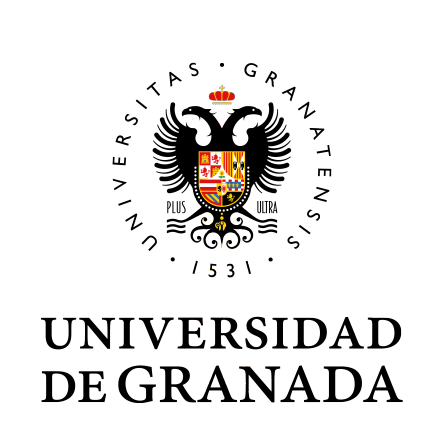
\includegraphics[scale=0.5]{img/ugr.png}\\

\textsc{\Large \asignatura{}\\[0.2cm]}
\textsc{GRADO EN INGENIERÍA INFORMÁTICA}\\[1cm]

\noindent\rule[-1ex]{\textwidth}{1pt}\\[1.5ex]
\textsc{{\Huge \titulo\\[0.5ex]}}
\textsc{{\Large \subtitulo\\}}
\noindent\rule[-1ex]{\textwidth}{2pt}\\[3.5ex]

\end{minipage}

\vspace{0.5cm}

\begin{minipage}{\textwidth}

\centering

\textbf{Autores}\\ {\autorv{}}\\{\autorj{}}\\{\autorf{}}\\[2.5ex]
\textbf{Rama}\\ {Computación y Sistemas Inteligentes}\\[2.5ex]
\vspace{0.3cm}


\includegraphics[scale=0.3]{img/etsiit.jpeg}

\vspace{0.5cm}
\textsc{Escuela Técnica Superior de Ingenierías Informática y de Telecomunicación}\\
\vspace{0.5cm}
\textsc{Curso 2019-2020}
\end{minipage}
\end{titlepage}

\pagenumbering{arabic}
\tableofcontents
\thispagestyle{empty}				% No usar estilo en la pagina de indice

\newpage

\setlength{\parskip}{1em}


\section{Introducción}
En este proyecto vamos a explicar nuestra \textit{Natural User Interface (NUI)} que hará que nuestra visita a la Alhambra sea más
dinámica y productiva. El proyecto constaría de varios dispositivos, como pueden ser principalmente unas gafas de realidad aumentada,
un dispositivo \textit{Leap Motion} y un micrófono integrados en las gafas, y un \textit{smartphone} que utilizaremos tanto para
manejar el sistema gracias a los múltiples sensores que incorpora como para controlar la aplicación.

En esta primera versión del proyecto vamos a encargarnos de la interfaz por sensores, es decir, dejaremos a un lado el \textit{Leap Motion}
y el controlador por voz. Vamos a encargarnos de la realidad aumentada y el resto de sensores para manejar el sistema.

\section{Interfaz por sensores}

Como no disponemos de unas gafas con estas características, simularemos su funcionamiento en la propia aplicación, utilizando un visor
VR con una imagen 3D del Patio de los Arrayanes y un lector de código QR. La idea es que estas dos características fuesen una sola, en
la cámara de las gafas. Por otro lado, llevaremos el \textit{smartphone} en la mano para controlar el contenido mostrado en las gafas, y
además, mostrará una maqueta de la Alhambra que nos servirá como mapa.

\subsection{Descripción del visor VR}
\label{sec:vr}

Por defecto, la aplicación lanza el \textbf{MainActivity} [\ref{sec:main}], inicializando la aplicación y mostrando el \textbf{ViewARFragment}
[\ref{sec:view}] (nuestro visor VR). El visor muestra una imagen de 360º, en la cual, cuando estemos mirando una estructura en concreto
(ya sea un edificio, puertas, columnas, jarrones, etc.), se nos marcará indicando que podremos interaccionar con ella.
Si movemos ligeramente el móvil hacia abajo cuando una de ellas esté resaltada, iniciamos la \textbf{InfoActivity} [\ref{sec:info}],
que es una pequeña página que muestra información extra sobre la estructura, como si fuese una enciclopedia. En nuestra aplicación esto
puede suponer un problema, ya que el visor lo tenemos en el móvil y al realizar el movimiento podemos deseleccionar lo que teníamos
resaltado; sin embargo, como esto estaría integrado en las gafas, cuando movamos el móvil, las gafas (que es donde vemos el objeto) no
se verán afectadas.

Una vez en el \textbf{InfoActivity}, para volver al visor VR, realizaremos un movimiento horizontal con nuestro dispositivo.
En nuestra aplicación, todo esto aparece en el dispositivo, pero en la versión definitiva, toda la información se mostraría en
las gafas.

\subsection{Descripción del lector QR}

En el menú desplegable, también tenemos la opción de \textit{Camera}, que nos lleva al \textbf{CameraFragment} [\ref{sec:camera}]. Este
implementa el lector de códigos QR, el cuál nos servirá a la hora de entrar a un edificio. Habrá códigos QR en cada uno y se obtendrá un
plano del edificio ya que las señales GPS pueden fallar o simplemente que el edificio tenga varias plantas y necesitemos ubicarnos mejor.
Cuando leemos un código se nos iniciará un \textbf{BlueprintsActivity}, que muestra la información anterior. Al igual que antes, para
volver a la cámara, realizaremos un movimiento horizontal con nuestro dispositivo.

\subsection{Descripción del mapa}
\label{sec:mapa}

Por último, en el menú desplegable tenemos un apartado llamado \textit{Navigation}, el cual inicia el \textbf{NavigationFragment} [\ref{sec:nav}]
quecnos muestra un maquetado 3D de toda la Alhambra con regiones clickables señaladas para saber en que lugar nos encontramos o si queremos
ir a algún otro lugar. Esta parte será la única que se vea en el smartphone. Tendremos implementados en él, el siguiente multitouch:

\begin{itemize}
    \item \textbf{Click simple}. Servirá para seleccionar y deseleccionar las regiones clickables.
    \item \textbf{Click simple arrastable}. Nos permite desplazarnos por el mapa.
    \item \textbf{Doble click}. Hacemos zoom en el mapa un valor predeterminado.
    \item \textbf{Pellizcar}. Ampliamos y alejamos la zona del mapa, dependiendo de hacia donde pellizquemos.
    \item \textbf{Click con dos dedos y arrastre}. Entramos en el modo 3D del mapa. En él nos desplazaremos como acabamos de ver.
    \item \textbf{Click con dos dedos y rotación}. Estando en el modo 3D, esto nos servirá para rotar la vista alrededor de la maqueta.
\end{itemize}

Como podemos ver, utilizamos bastantes sensores multitouch, pero no hay ninguno que requiera del acelerómetro, giroscopio, etc., por lo
que no tendremos colisiones entre éste y los mencionados anteriormente.



% start new page before setting page layout,
% otherwise previous page is also affected
\KOMAoption{paper}{landscape}%
\typearea{12}% sets new DIV

% Establecer pagina horizontal
\recalctypearea
% needed to show page in landscape in viewer
\pdfpageheight=\paperheight
\pdfpagewidth=\paperwidth
% Poner estilo
\pagestyle{lscape}

\newpage

\section{Diagrama de clases}

A continuación se puede ver el diagrama de clases. No se han incluido atributos ni métodos porque se van a describir más adelante.

\begin{figure}[H]
\centering
\begin{tikzpicture}[scale=0.7]
	\begin{class}[text width=3cm]{MainActivity}{0,0}
	\end{class}
	
	\begin{class}[text width=4cm]{CameraFragment}{-9, -5}
	\end{class}
	\begin{class}[text width=3cm]{ExitFragment}{-7, -1}
	\end{class}
	\begin{class}[text width=5cm]{NavigationFragment}{0, -6.5}
	\end{class}
	\begin{class}[text width=4cm]{ViewARFragment}{9, -5}
	\end{class}
	\begin{class}[text width=4cm]{BlueprintsActivity}{-9, -9}
	\end{class}
	\begin{class}[text width=3cm]{InfoActivity}{9, -9}
	\end{class}
	
	\unidirectionalAssociation{MainActivity}{}{1}{CameraFragment}
	\unidirectionalAssociation{MainActivity}{}{1}{ExitFragment}
	\unidirectionalAssociation{MainActivity}{}{1}{NavigationFragment}
	\unidirectionalAssociation{MainActivity}{}{1}{ViewARFragment}
	
	\draw[umlcd style dashed line,->] (ViewARFragment) -- node[above, sloped, black] {$<<$uses$>>$} (InfoActivity);
	\draw[umlcd style dashed line,->] (CameraFragment) -- node[above, sloped, black] {$<<$uses$>>$} (BlueprintsActivity);
\end{tikzpicture}
\caption{Diagrama de clases simplificado.}
\label{fig:class-diagram}
\end{figure}

\KOMAoptions{paper=portrait}
\recalctypearea
\pdfpageheight=\paperheight
\pdfpagewidth=\paperwidth
\headwidth\textwidth

\section{Descripción de las clases}

Una vez visto el diagrama de clases, vamos a proceder a comentar brevemente qué es lo que hace cada clase, sus
atributos, y sus métodos.

\subsection{\textbf{MainActivity}}
\label{sec:main}

Es la actividad principal, encargada de construir la barra de actividades que permite acceder
a los \textit{fragments} y de solicitar los permisos de cámara y localización necesarios para ejecutar
la aplicación.

\subsubsection{Atributos}

Los atributos que tiene esta clase son los siguientes:

\begin{itemize}
    \item 
\end{itemize}

\subsubsection{Métodos}


\subsection{\textbf{ExitFragment}}
\label{sec:exit}

\textit{Fragment} que pregunta al usuario si quiere salir o no de la aplicación y, en caso afirmativo, la cierra.

\subsubsection{Atributos}

\subsubsection{Métodos}

\subsection{\textbf{CameraFragment}}
\label{sec:camera}

\textit{Fragment} que permite acceder al sensor de la cámara para poder realizar la lectura
de códigos QR. Una vez leídos, se encarga también de pasarlos a \textbf{BlueprintActivity} para que éste los procese.
Para la detección y lectura de los códigos QR se utiliza la biblioteca \textit{BarcodeDetector}.

\subsubsection{Atributos}

\subsubsection{Métodos}

\subsection{\textbf{NavigationFragment}}
\label{sec:nav}

\textit{Fragment} que permite acceder a un mapa de la Alhambra y navegar por él, destacando
algunos de los edificios y permitiendo interactuar con ellos, tal y como se ha descrito en la sección \ref{sec:mapa}.
Para poder trabajar con mapas, se utiliza la API de GoogleMaps.

\subsubsection{Atributos}

\subsubsection{Métodos}

\subsection{\textbf{ViewARFragment}}
\label{sec:view}

\textit{Fragment} que simula la visión en realidad aumentada del interior de los Palacios
Nazaríes. Simula que detecta zonas interesantes y las destaca. Cuando se realiza un gesto con el dispositivo, tal y como se
ha indicado en la sección \ref{sec:vr}, muestra más información sobre el elemento destacado, utilizando para ello la clase
\textbf{InfoActivity}.

\subsubsection{Atributos}

\subsubsection{Métodos}

\subsection{\textbf{BluePrintsActivity}}
\label{sec:blue}

Actividad que se encarga de recibir las lecturas QR de \textbf{CameraFragment} y de procesarlas, mostrando la información
correspondiente a la lectura.

\subsubsection{Atributos}

\subsubsection{Métodos}

\subsection{\textbf{InfoActivity}}
\label{sec:info}

Actividad que muestra información sobre la zona que ha sido destacada en \textbf{ViewARFragment}.
Procesa la información que tiene ésta y muestra una u otra información.

\subsubsection{Atributos}
\subsubsection{Métodos}



\newpage

\begin{thebibliography}{5}

\bibitem{nombre-referencia}
Texto referencia
\\\url{https://url.referencia.com}

\end{thebibliography}

\end{document}

